\section{Ejercicio 1}

\begin{figure}[H]
\centering
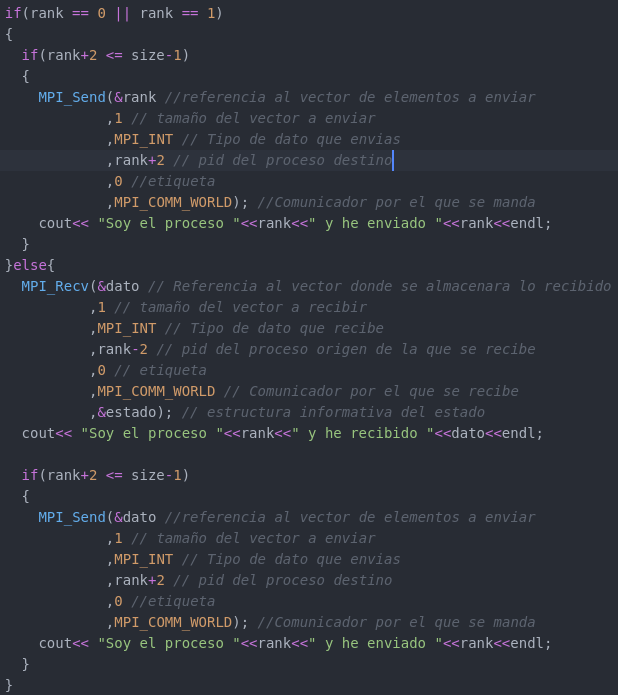
\includegraphics[width=0.8\textwidth]{imagenes/ej1.png}
\end{figure}

He añadido los ifs correspondientes para que solo los proceso 0 y 1 envíen sus \textit{ids}(solo cuando haya mas procesos pares o impares) y los correspondientes reciban ese \textit{id}(y envien al siguiente cuando proceda).

\section{Ejercicio 2}

\begin{figure}[H]
\centering
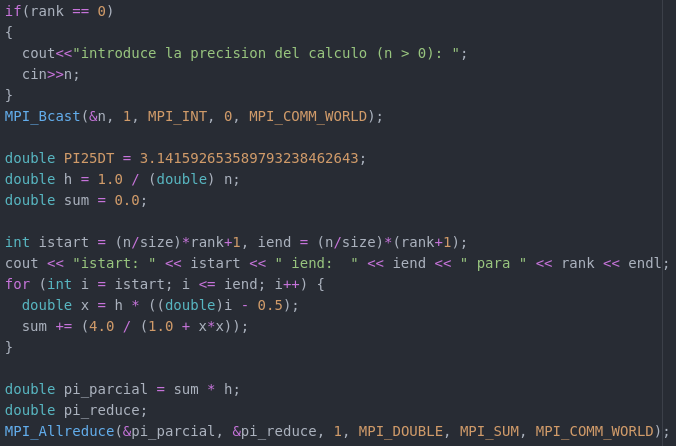
\includegraphics[width=0.8\textwidth]{imagenes/ej2.png}
\end{figure}

Se difunde el valor introducido por teclado al resto de procesos. Luego, cada proceso calcula su intervalo y se reduce para todos ya que se pide que la solución se obtenga para todos los procesos.

\section{Ejercicio 3}

\begin{figure}[H]
\centering
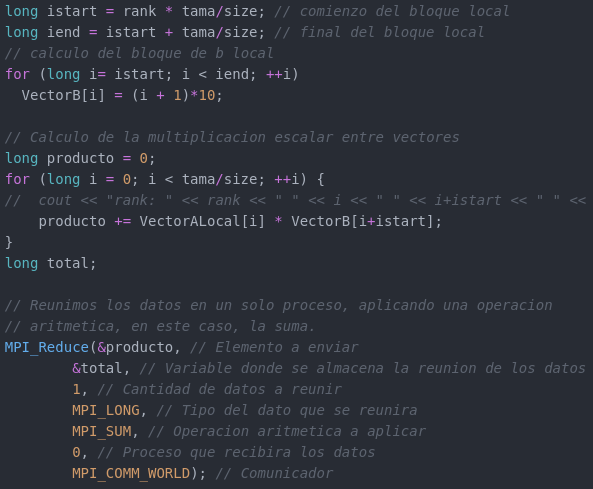
\includegraphics[width=0.8\textwidth]{imagenes/ej3.png}
\end{figure}

Para el vectorB, ahora se inicializa cada segmento \textit{$s_i$} por el proceso \textit{$p_i$} y el producto lo hace cada proceso multiplicando su vectorA local por su segmento \textit{$s_i$} del vectorB.

\section{Ejercicio 4}

\begin{figure}[H]
\centering
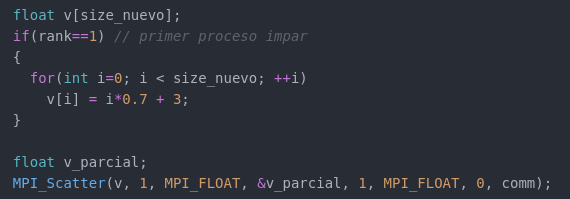
\includegraphics[width=0.8\textwidth]{imagenes/ej4.png}
\end{figure}

Dejo que el primer proceso impar(rank global = 1) inicialice el vector y se reparten al resto de impares usando el comunicador \textit{comm} con color=rank\%2. Así el root 0, que corresponde al primero de los impares lo reparte al resto. 